\section{Experimental Setup}

For the analysis of a DDPG network was used the programming language Python \cite{ascher1999learning}. 
The Python language has as priority the legibility of the code under speed. 
The vast library and frameworks provided by Python makes it an exquisite tool for machine learning and data analysis purposes.

\subsection{ROS}

The robot operations system (ROS) is a flexible framework to write software for robots.
ROS \cite{pyo2015ros} is a collection of tools, and libraries.
ROS provides operational system's standard services, like hardware's abstraction, device low level control, messages between processes and package management. 
The set of ROS processes in execution are represented by graphs architecture where the processing is performed on nodes that receive and send messages as sensors, control, state, planning, actuator and others.

Despite the importance of low latency on the robots control, ROS is not a real-time operational system, although it is possible to integrate ROS with real-time code. This lack of real-time system is being addressed on the development of ROS 2.0.

\subsection{TurtleBot}

TurtleBot is a ROS standard platform robot, and there are 3 version of the series. TurtleBots are affordable and programmable mobile robots for use in education, research, hobby, and product prototyping.
The third version was used on this project, shown in Fig. \ref{fig:turtlebot3}.

\begin{figure}[htbp]
\centerline{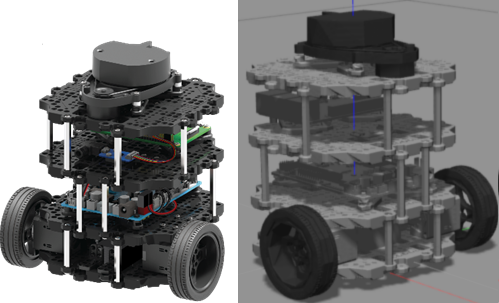
\includegraphics[width=\columnwidth]{images/burger.png}}
\caption{Real and simulated TurtleBot3 Burger in Gazebo.}
\label{fig:turtlebot3}
\end{figure}

The TurtleBot3 Burger uses 2 DYNAMIXEL motord series XL, for the object detection the TurtleBot3 utilize a 360 degree sensor laser LiDAR, and it has an IMU sensor for the odometry calculations.
All the control is made by the open source controller board OpenCR1.0 and Raspberry Pi 3 microprocessor.
% The Table \ref{tab1} shows all hardware specification of the TurtleBot3 version Burger.


% \begin{table}[htbp]
% \caption{Hardware Specication of the TurtleBot3 Burger}
% \begin{center}
% \begin{tabular}{|c|c|}
% \hline
% \textbf{Items}&\textbf{Specification} \\
% \hline
% Maximum translational velocity & 0.22 m/s \\
% \hline
% Maximum rotational velocity    & 2.84 rad/s (162.72 deg/s) \\
% \hline
% Maximum payload                & 15kg \\ 
% \hline
% Size (L x W x H)               & 138mm x 178mm x 192mm \\
% \hline
% Weight                         & 1kg \\
% \hline
% Threshold of climbing          & 10 mm or lower \\
% \hline
% Expected operating time        & 2h 30m \\
% \hline
% Expected charging time         & 2h 30m \\
% \hline
% SBC (Single Board Computers)   & Raspberry Pi 3 Model B and B+ \\
% \hline
% Actuator                       & DYNAMIXEL XL430-W250 \\
% \hline
% LDS(Laser Distance Sensor)     & 360 Laser Distance Sensor LDS-01 \\
% \hline
% IMU                            & \begin{tabular}[c]{@{}c@{}}Gyroscope 3 Axis\\ Accelerometer 3 Axis\\ Magnetometer 3 Axis\end{tabular} \\
% \hline
% Battery                        & \begin{tabular}[c]{@{}c@{}}Lithium polymer \\ 11.1V 1800mAh / 19.98Wh 5C \\ \end{tabular} \\
% \hline

% \end{tabular}
% \label{tab1}
% \end{center}
% \end{table}

\subsection{Gazebo}

Robot simulation is an essential tool on all roboticist's toolbox.
A good simulator makes possible to test algorithms quickly, to design robots, and to train systems with artificial intelligence using realistic scenarios.
With Gazebo \cite{fairchild2016ros} is possible to simulate this environments easily and with the advantage of having an active community.
This makes Gazebo a great tool on the area of robotic simulation.
